\documentclass[9pt,a5paper]{extarticle}
\usepackage[margin=.75cm]{geometry}
\usepackage[utf8]{inputenc}
\usepackage[IL2]{fontenc}
\usepackage[czech]{babel}
\usepackage{microtype}
\usepackage{amssymb}
\usepackage{amsthm}
\usepackage{amsmath}
\usepackage{xcolor}
\usepackage{graphicx}
\usepackage{wasysym}
\usepackage{tikz}

\usepackage[inline]{enumitem}

\newcommand{\R}{\mathbb{R}}

\newcommand{\hint}[1]{{\color{gray}\footnotesize\noindent(Nápověda: #1)}}

\setlist[enumerate]{label={(\alph*)},topsep=\smallskipamount,itemsep=\smallskipamount,parsep=0pt}
\setlist[itemize]{topsep=\smallskipamount,noitemsep}

\def\tisk{%
\newbox\shipouthackbox
\pdfpagewidth=2\pdfpagewidth
\let\oldshipout=\shipout
\def\shipout{\afterassignment\zdvojtmp \setbox\shipouthackbox=}%
\def\zdvojtmp{\aftergroup\zdvoj}%
\def\zdvoj{%
    \oldshipout\vbox{\hbox{%
        \copy\shipouthackbox
        \hskip\dimexpr .5\pdfpagewidth-\wd\shipouthackbox\relax
        \box\shipouthackbox
    }}%
}}%



\newtheorem*{poz}{Pozorování}

\theoremstyle{definition}
\newtheorem{uloha}{\atr Úloha}
\newtheorem{suloha}[uloha]{\llap{$\star$ }Úloha}
\newtheorem*{bonus}{Bonus}
\newtheorem*{defn}{Definice}

\pagestyle{empty}

\let\ee\expandafter

\def\vysld{}
\let\printvysl\relax
\let\printalphvysl\relax

\makeatletter
\long\def\vyslplain#1{\ee\ee\ee\gdef\ee\ee\ee\vysld\ee\ee\ee{\ee\vysld\ee\printvysl\ee{\the\c@uloha}{#1}}}

\def\locvysl#1{\ee\gdef\ee\locvysld\ee{\locvysld\item #1}}
\let\lv\locvysl

\newenvironment{ulohav}[1][]{\begin{uloha}[#1]\gdef\locvysld{\begin{enumerate}}}{\ee\vyslplain\ee{\locvysld\end{enumerate}}\end{uloha}}
\def\stitem{\@noitemargtrue\@item[$\star$ \@itemlabel]}

\makeatother

\def\atr{}
\def\basic{\def\atr{\llap{\mdseries$\sun$ }\gdef\atr{}}}

\begin{document}


%\tisk


\section*{8. Trénink souřadnic}

\begin{ulohav}
\[\begin{tikzpicture}[x=.6cm,y=.6cm]
\draw[help lines, color=gray, dashed] (-5,-5) grid[step=1] (5,5);
\draw[->,thick] (-5,0)--(5,0) node[right]{$x$};
\draw[->,thick] (0,-5)--(0,5) node[above]{$y$};
\node[below left] at (0,0) {$O$};

\draw[->,thick,densely dashed] (-5,-2)--(5,-2) node[right]{$x'$};
\draw[->,thick,densely dashed] (-3,-5)--(-3,5) node[above]{$y'$};
\node[below left] at (-3,-2) {$O'$};
\end{tikzpicture}\]
\begin{enumerate}
    \item V soustavě souřadnic $Oxy$ vyznačte body $A[-1; 2]$ a $B[3; -3]$.\lv{--}
    \item Určete souřadnice bodů $A$, $B$ v soustavě souřadnic $O'x'y'$.\lv{$A[2; 4]$, $B[6; -1]$}
    \item Spočtěte souřadnice středu úsečky $AB$ v $Oxy$.\lv{$S_{AB}[1; -\frac12]$}
    \item Spočtěte souřadnice středu úsečky $AB$ v $O'x'y'$.\lv{$S_{AB}[4; \frac32]$}
    \item Spočtěte souřadnice \uv{součtu bodů} $A$ a $B$ v $Oxy$, výsledný bod vyznačte.\lv{$A+B[2; -1]$}
    \item Spočtěte souřadnice \uv{součtu bodů} $A$ a $B$ v $O'x'y'$, výsledný bod vyznačte.\lv{$A+B[8; 3]$}
    \item Vyvoďte z předchozích dvou podúloh závěr o smysluplnosti \uv{sčítání bodů}.\lv{Nemá to \emph{geometrický} význam, protože výsledek (na rozdíl od středu) záleží na zvolené soustavě souřadnic.}
    \item Existuje bod, který by měl tytéž souřadnice v $Oxy$ jako v $O'x'y'$?\lv{Ne, protože jedny souřadnice se z druhých spočtou jenom přičtením nějakých čísel, tedy se vždycky změní.}
    \item Nalezněte všechny body $X$, které budou mít v $Oxy$ obě souřadnice stejné a jejich vzdálenost od bodu $A$ bude $\sqrt{17}$. Vyznačte si je a rozmyslete si, co jste \uv{geometricky} provedli.\lv{dvě řešení: $X_1[-2; -2]$, $X_2[3; 3]$.}
\end{enumerate}
\end{ulohav}


\begin{ulohav}
V prostoru jsou dány body $A[0;4;0]$, $B[4;4;0]$, $C[?;0;0]$, $A'[?;?;4]$.
\begin{enumerate}
    \item Doplňte zbývající souřadnice u vrcholů krychle $ABCDA'B'C'D'$.\lv{$C[4;0;0]$, $D[0;0;0]$, $A'[0;4;4]$, $B'[4;4;4]$, $C'[4;0;4]$, $D'[0;0;4]$}
    \item Zakreslete body do soustavy souřadnic $Oxyz$.\lv{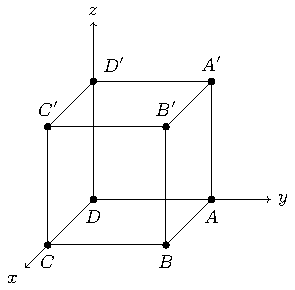
\includegraphics{krychle.pdf}}
    \item Spočítejte vzdálenost $|A'K|$, kde $K$ je střed úsečky $AD$.\lv{$2\sqrt5$}
    \item Spočítejte vzdálenost $|MN|$, kde $M$ je střed úsečky $AA'$ a $N$ je střed úsečky $KC$.\lv{$\sqrt{17}$}
\end{enumerate}
\end{ulohav}


\begin{ulohav}
Rozmyslete si, jak se budou měnit souřadnice bodů v rovině, pokud je budeme
\begin{enumerate}
    \item zobrazovat v osové souměrnosti podle osy $x$,\lv{$y$-ová souřadnice změní znaménko}
    \item zobrazovat v osové souměrnosti podle osy $y$,\lv{$x$-ová souřadnice změní znaménko}
    \item zobrazovat v osové souměrnosti podle přímky $y = x$,\lv{prohodí se souřadnice}
    \item zobrazovat v osové souměrnosti podle přímky $y = -x$,\lv{prohodí se souřadnice a obě změní znaménko}
    \item rotovat kolem počátku o $180^\circ$,\lv{obě souřadnice změní znaménko}
    \item rotovat kolem počátku o $90^\circ$ proti směru ručiček,\lv{prohodí se souřadnice a pak $x$-ová změní znaménko (ne naopak!)}
    \stitem rotovat kolem počátku o $45^\circ$ proti směru ručiček.\lv{ze souřadnic $[a;b]$ se stanou $\bigl[\frac{a}{\sqrt{2}}-\frac{b}{\sqrt{2}}; \frac{a}{\sqrt{2}}+\frac{b}{\sqrt{2}}\bigr]$}
\end{enumerate}
\end{ulohav}



\newpage
\parindent=0pt
\parskip=\smallskipamount
\def\printvysl#1#2{\textbf{#1.}\ #2\par}
\vysld


\end{document}